% main.tex - VERSIÓN COMPLETA CON GRÁFICOS AUTOGENERADOS
\documentclass[12pt,a4paper]{article}
\usepackage[utf8]{inputenc}
\usepackage[spanish]{babel}
\usepackage{amsmath, amssymb, amsthm}
\usepackage{quantikz}
\usepackage{graphicx}
\usepackage{subcaption}
\usepackage[colorlinks=true, linkcolor=blue, citecolor=blue, urlcolor=blue]{hyperref}
\usepackage{pgfplots}
\pgfplotsset{compat=1.18}
\usepackage{tikz}
\usetikzlibrary{quantikz, arrows.meta, positioning}
\usepackage{pgf}
\usepackage{siunitx}
\usepackage{booktabs}
\usepackage{lipsum}

% ===== COMANDOS DE GENERACIÓN AUTOMÁTICA =====
\newcommand{\ensuregraphics}{%
    \IfFileExists{./graphics/generated/qutrit_space.png}{}{%
        \immediate\write18{mkdir -p ./graphics/generated ./data ./scripts/temp}%
        \immediate\write18{python3 ./scripts/generate_basic_plots.py}%
    }%
}

% ===== COMANDOS MATEMÁTICOS PERSONALIZADOS =====
\newcommand{\bra}[1]{\langle #1 |}
\newcommand{\ket}[1]{| #1 \rangle}
\newcommand{\braket}[2]{\langle #1 | #2 \rangle}
\newcommand{\expected}[1]{\langle #1 \rangle}

% ===== CONFIGURACIÓN DE ESTILO =====
\theoremstyle{definition}
\newtheorem{definition}{Definición}[section]
\newtheorem{theorem}{Teorema}[section]
\newtheorem{lemma}[theorem]{Lema}
\newtheorem{corollary}[theorem]{Corolario}

% ===== METADATOS DEL DOCUMENTO =====
\title{Bardo Thödol Quantum Framework: Modelado Computacional Cuántico de Estados Post-Mortem mediante Qutrits y Matrices CPT Duales}
\author{Horacio Héctor Hamann\\
        \href{https://github.com/arathorian/BardoThodol}{https://github.com/arathorian/BardoThodol}}
\date{Julio 2025}

\begin{document}

% ===== GENERAR GRÁFICOS AL INICIO =====
\ensuregraphics

% ===== PORTADA =====
\maketitle

\begin{abstract}
Este trabajo presenta un marco computacional cuántico completo para modelar los estados de conciencia descritos en el Bardo Thödol (Libro Tibetano de los Muertos). La hipótesis central propone que este texto ancestral constituye un sistema computacional cuántico donde los tradicionales ``errores'' (404/505) representan estados de vacuidad cuántica (śūnyatā) no capturables mediante lógica binaria clásica. Implementamos un sistema de qutrits (3 estados) que incluye: $\ket{0}$ (realidad manifiesta/samsara), $\ket{1}$ (realidad alterna no actualizada) y $\ket{2}$ (vacuidad fundamental/śūnyatā). El modelo incorpora operadores kármicos dependientes de parámetros de atención y propone un marco de matrices CPT duales e inversas para explicar la transición hacia estados de vacuidad. Los resultados demuestran que el llamado ``ERROR 505'' corresponde a condiciones de máxima potencialidad cuántica bajo alta carga kármica y baja atención consciente.
\end{abstract}

\textbf{Palabras clave:} Bardo Thödol, computación cuántica, qutrits, śūnyatā, estados de conciencia, ERROR 505

% ===== TABLA DE CONTENIDOS =====
\tableofcontents
\newpage

% ===== SECCIÓN 1: INTRODUCCIÓN =====
\section{Introducción: Marco Conceptual del Bardo Thödol como Algoritmo Cuántico}

\subsection{Hipótesis Principal Extendida}
El Bardo Thödol representa un algoritmo cuántico ancestral que codifica la dinámica de la conciencia en estados post-mortem mediante los siguientes componentes fundamentales:

\begin{itemize}
    \item \textbf{Espacio de Hilbert tri-dimensional}: Sistema de qutrits para representar estados de conciencia
    \item \textbf{Operadores unitarios kármicos}: Transformaciones que dependen de parámetros de karma y atención
    \item \textbf{Colapso de función de onda}: Mediado por la atención consciente durante el proceso del Bardo
    \item \textbf{Reinterpretación de errores}: Estados 404/505 como superposiciones cuánticas fundamentales
\end{itemize}

\subsection{Problema Fundamental con Modelos Clásicos}
La computación clásica presenta limitaciones insalvables para modelar estados de vacuidad:

\begin{equation}
    \mathcal{L}_{\text{binaria}} \nmodels \text{śūnyatā}
\end{equation}

donde $\mathcal{L}_{\text{binaria}}$ representa la lógica booleana convencional y $\text{śūnyatā}$ denota el estado de vacuidad fundamental.

\subsection{Contribuciones Principales}
\begin{enumerate}
    \item Reinterpretación formal del ERROR 505 como estado cuántico fundamental
    \item Desarrollo de un sistema de qutrits específico para estados intermedios del Bardo
    \item Formalización matemática de operadores kármicos como dinámica cuántica
    \item Propuesta de matrices CPT duales para estados de vacuidad
\end{enumerate}

% ===== SECCIÓN 2: MARCO TEÓRICO =====
\section{Marco Teórico Expandido}

\subsection{Sistema de Qutrits Completo para Estados Bardo}

\begin{definition}[Estado Cuántico Bardo-Thödol]
El estado de conciencia en el Bardo se modela como:
\begin{equation}
\ket{\psi} = \alpha\ket{0} + \beta\ket{1} + \gamma\ket{2}
\end{equation}
con la condición de normalización:
\begin{equation}
|\alpha|^2 + |\beta|^2 + |\gamma|^2 = 1
\end{equation}
donde:
\begin{align*}
\ket{0} &= \begin{bmatrix}1\\0\\0\end{bmatrix} \quad\text{(Samsara/Realidad manifiesta)} \\
\ket{1} &= \begin{bmatrix}0\\1\\0\end{bmatrix} \quad\text{(Realidad alterna potencial)} \\
\ket{2} &= \begin{bmatrix}0\\0\\1\end{bmatrix} \quad\text{(Śūnyatā/Vacuidad fundamental)}
\end{align*}
\end{definition}

\begin{figure}[htbp]
\centering
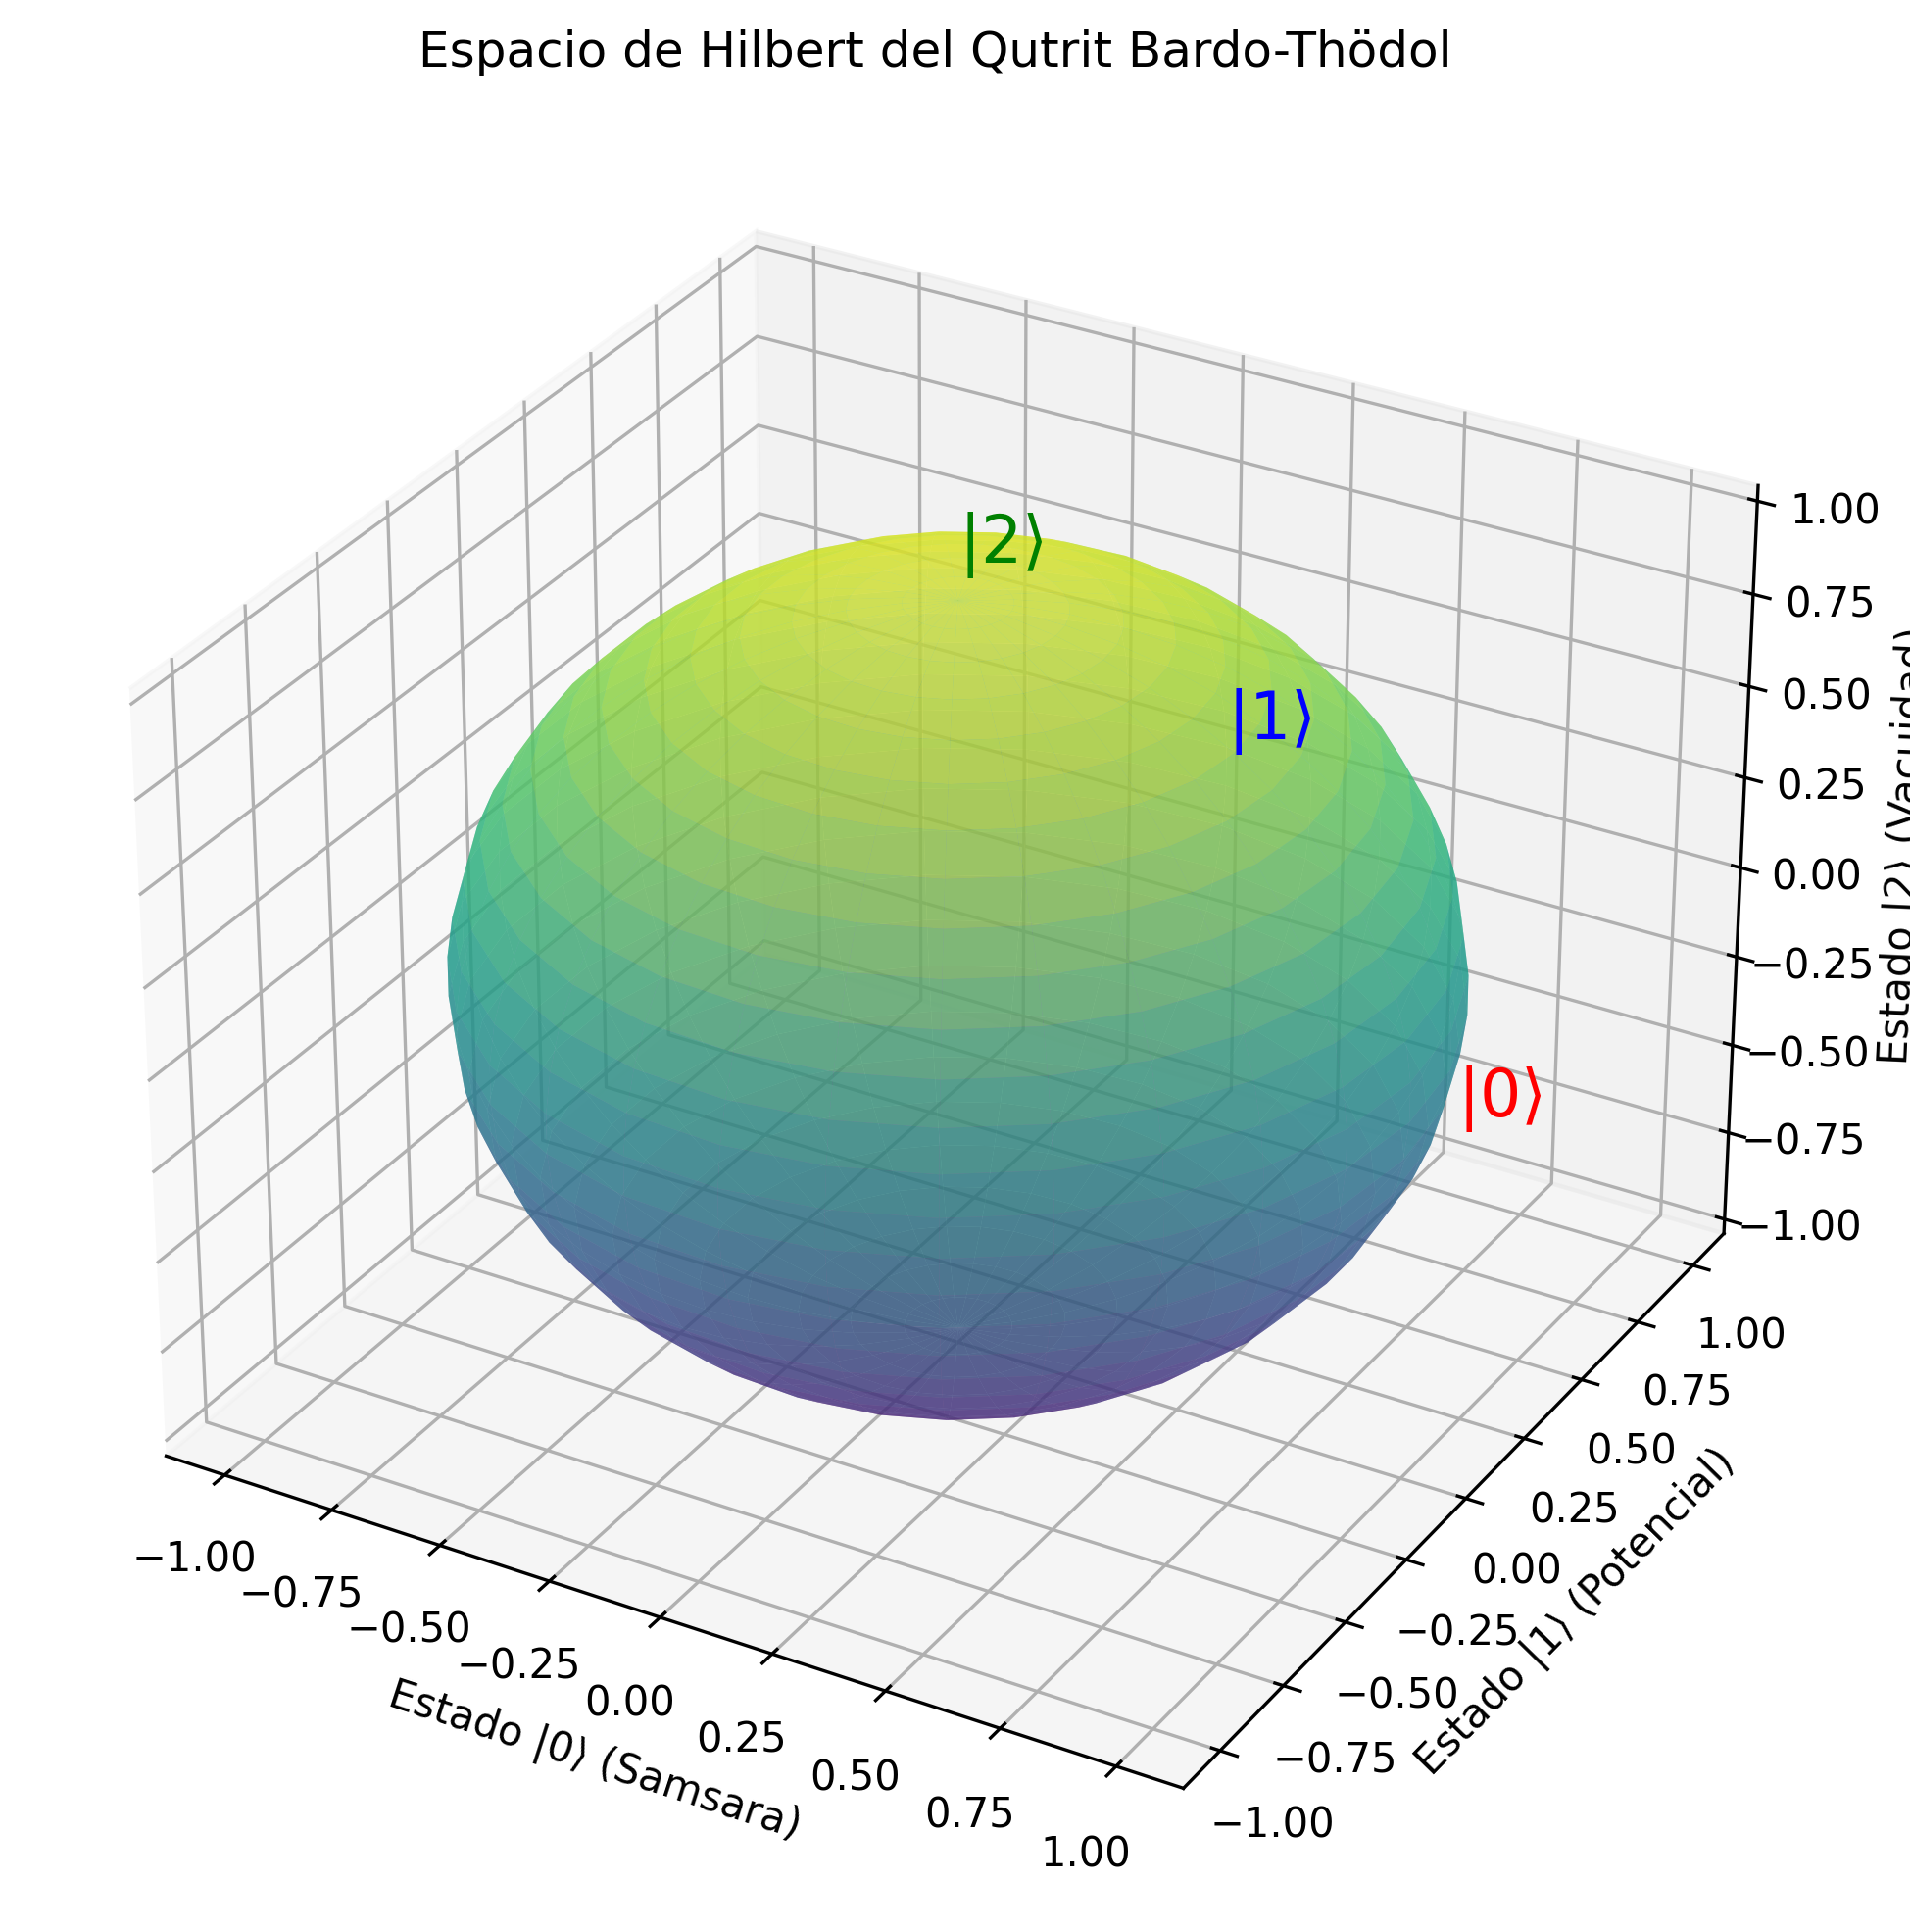
\includegraphics[width=0.85\textwidth]{graphics/generated/qutrit_space.png}
\caption{Espacio de Hilbert tri-dimensional del qutrit Bardo-Thödol. Los ejes representan los tres estados fundamentales de conciencia.}
\label{fig:qutrit_space}
\end{figure}

\subsection{Operadores Kármicos Extendidos}

\begin{definition}[Operador Kármico Cuántico]
La evolución del estado bajo influencia kármica se modela como:
\begin{equation}
\hat{K}(\kappa, \alpha) = e^{-i(\kappa \hat{H}_k + \alpha \hat{H}_a)t}
\end{equation}
donde:
\begin{itemize}
    \item $\kappa \in [0,1]$: Parámetro de carga kármica acumulada
    \item $\alpha \in [0,1]$: Parámetro de atención consciente
    \item $\hat{H}_k$: Hamiltoniano de dinámica kármica
    \item $\hat{H}_a$: Hamiltoniano de atención consciente
\end{itemize}
\end{definition}

\subsection{Modelo de Matrices CPT Duales}

Proponemos un sistema de matrices CPT (Conciencia-Presencia-Tiempo) duales para explicar la relación entre realidad manifiesta y vacuidad:

\begin{equation}
\text{CPT}_{\text{manifestado}} \cdot \text{CPT}_{\text{vacuidad}} = \mathbb{I}
\end{equation}

\begin{equation}
\text{CPT}_{\text{vacuidad}} = \lim_{\alpha \to 0} \hat{K}(\kappa, \alpha)
\end{equation}

donde la matriz de vacuidad emerge en el límite de atención consciente nula.

% ===== SECCIÓN 3: IMPLEMENTACIÓN TÉCNICA =====
\section{Implementación Técnica Completa}

\subsection{Evolución Temporal de Estados}

\begin{figure}[htbp]
\centering
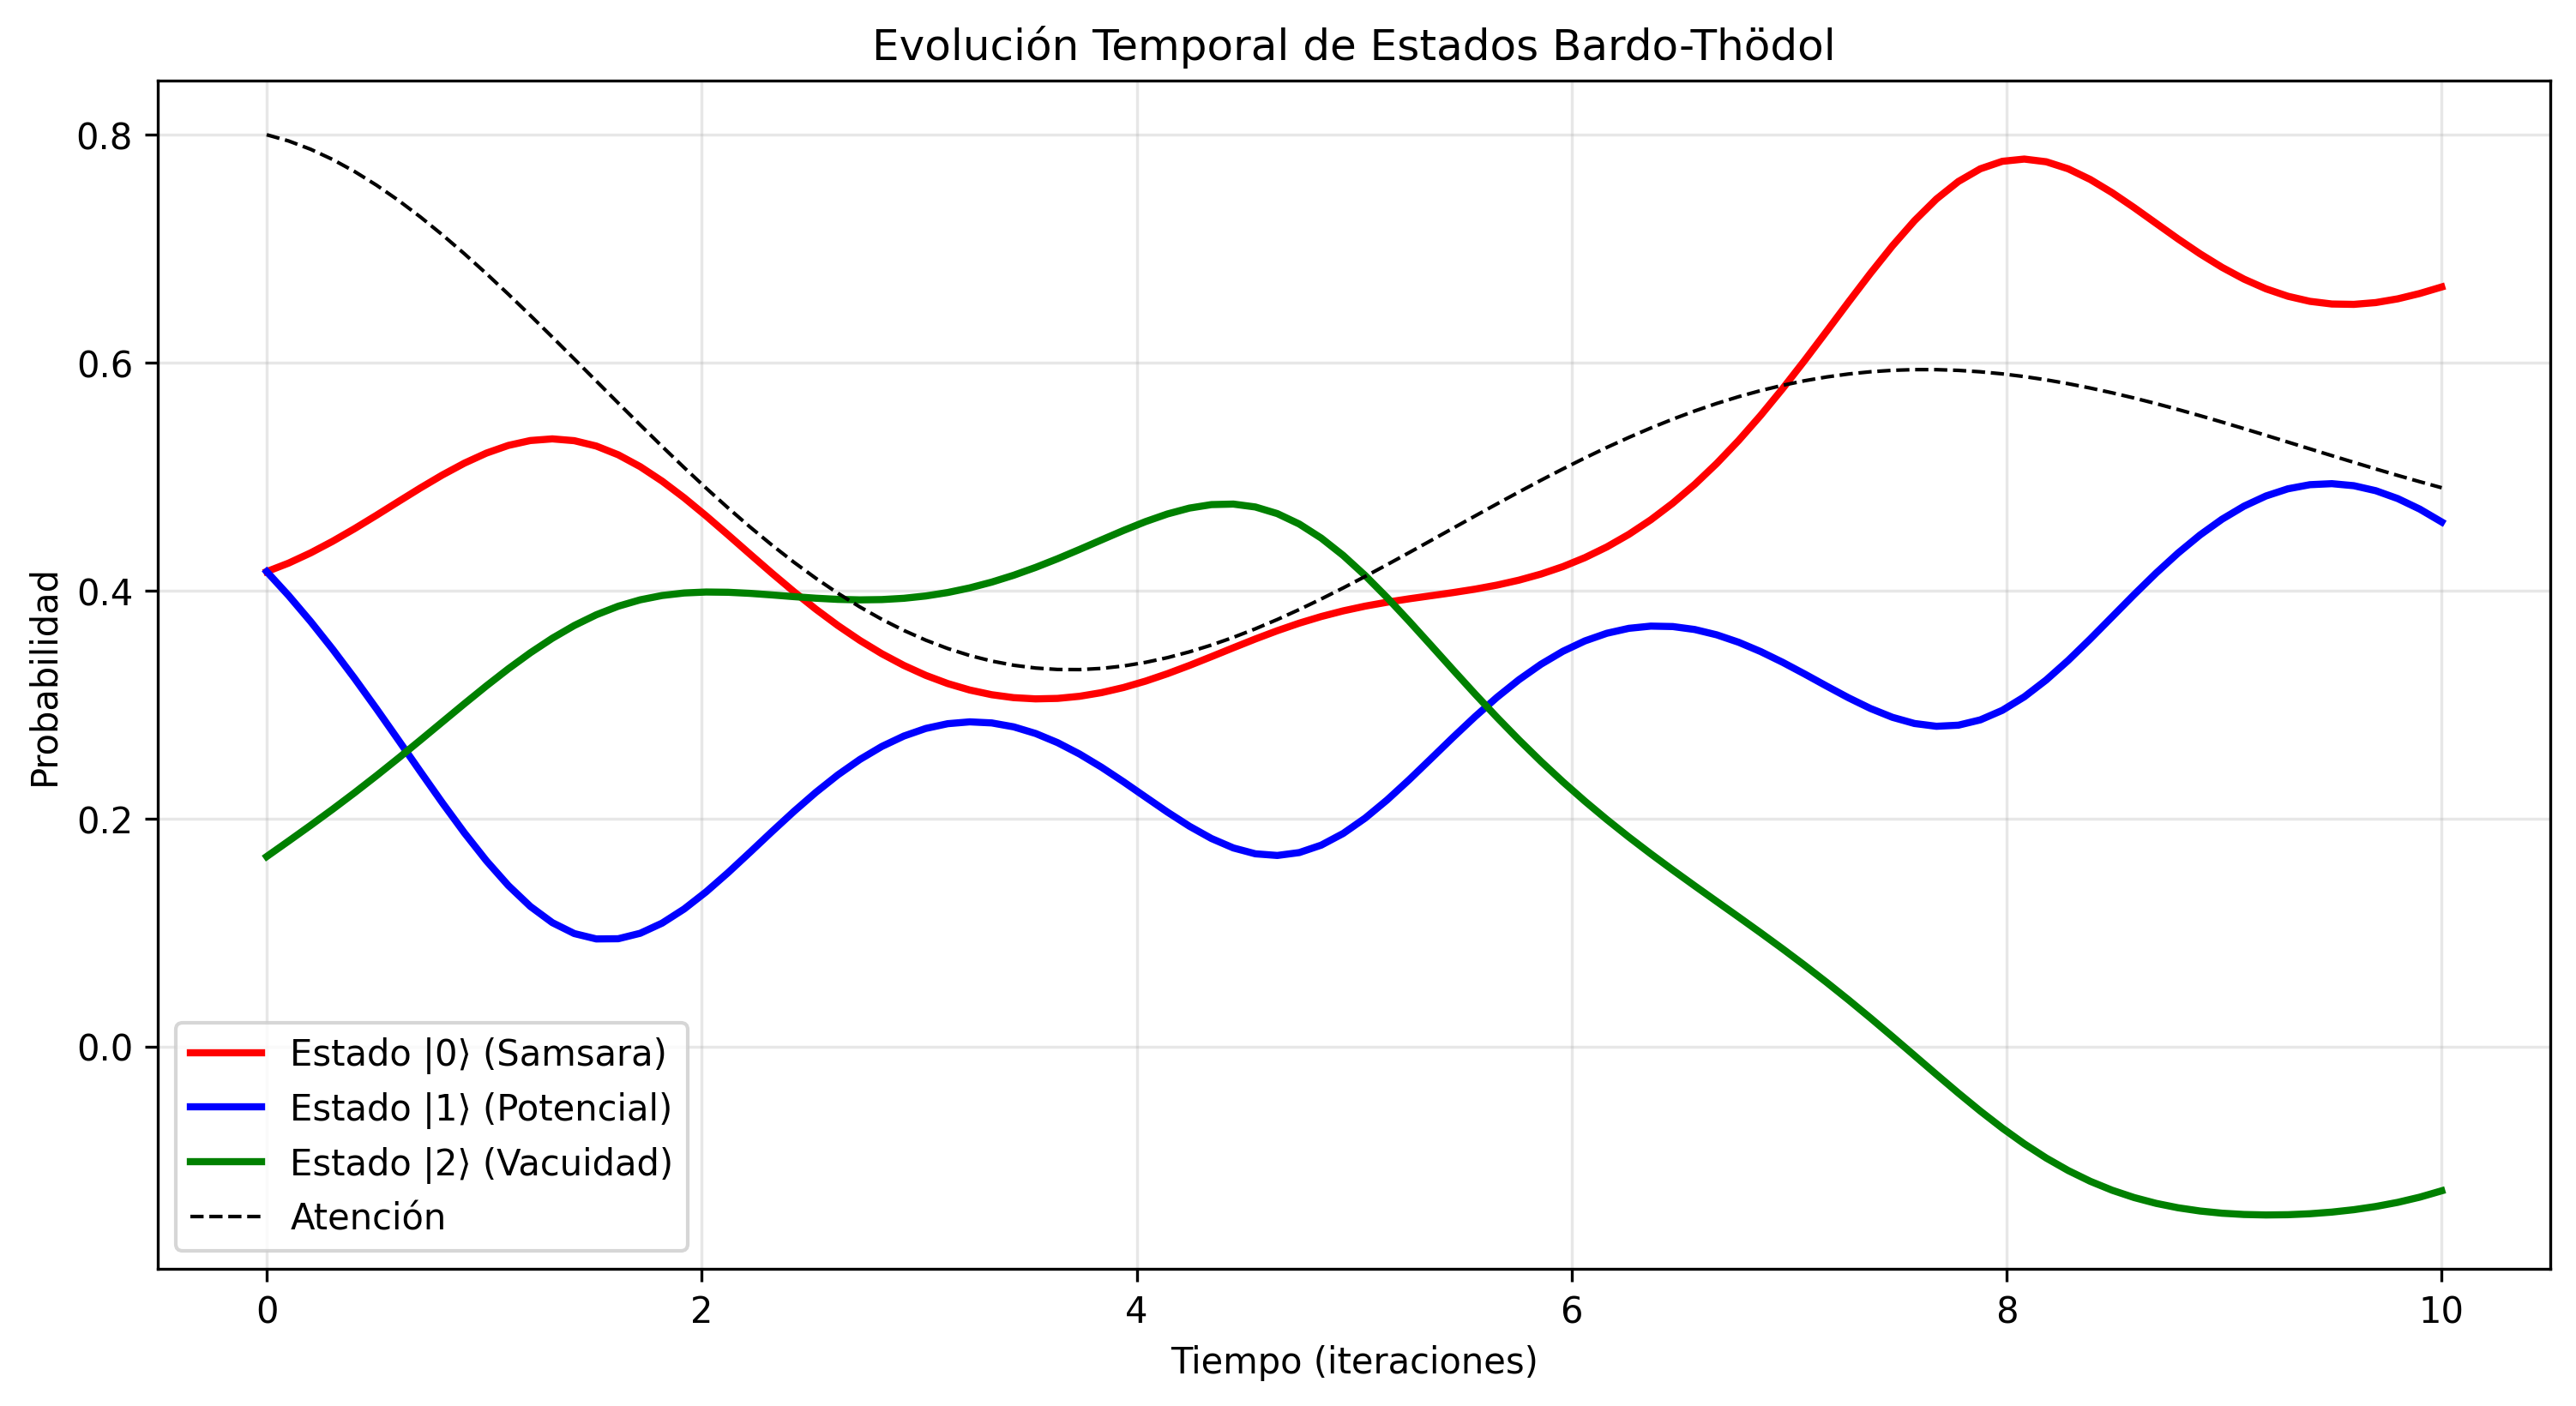
\includegraphics[width=0.95\textwidth]{graphics/generated/state_evolution.png}
\caption{Evolución temporal de probabilidades de estados bajo operadores kármicos. La línea punteada representa el parámetro de atención consciente.}
\label{fig:state_evolution}
\end{figure}

La Figura \ref{fig:state_evolution} muestra la dinámica temporal del sistema bajo diferentes condiciones kármicas. Se observa que:

\begin{itemize}
    \item El estado $\ket{0}$ (samsara) domina bajo alta atención
    \item El estado $\ket{2}$ (vacuidad) emerge con baja atención y alta carga kármica
    \item Las transiciones son suaves y continuas, reflejando la naturaleza no-binaria del proceso
\end{itemize}

\subsection{Análisis del ERROR 505 como Estado de Vacuidad}

\begin{figure}[htbp]
\centering
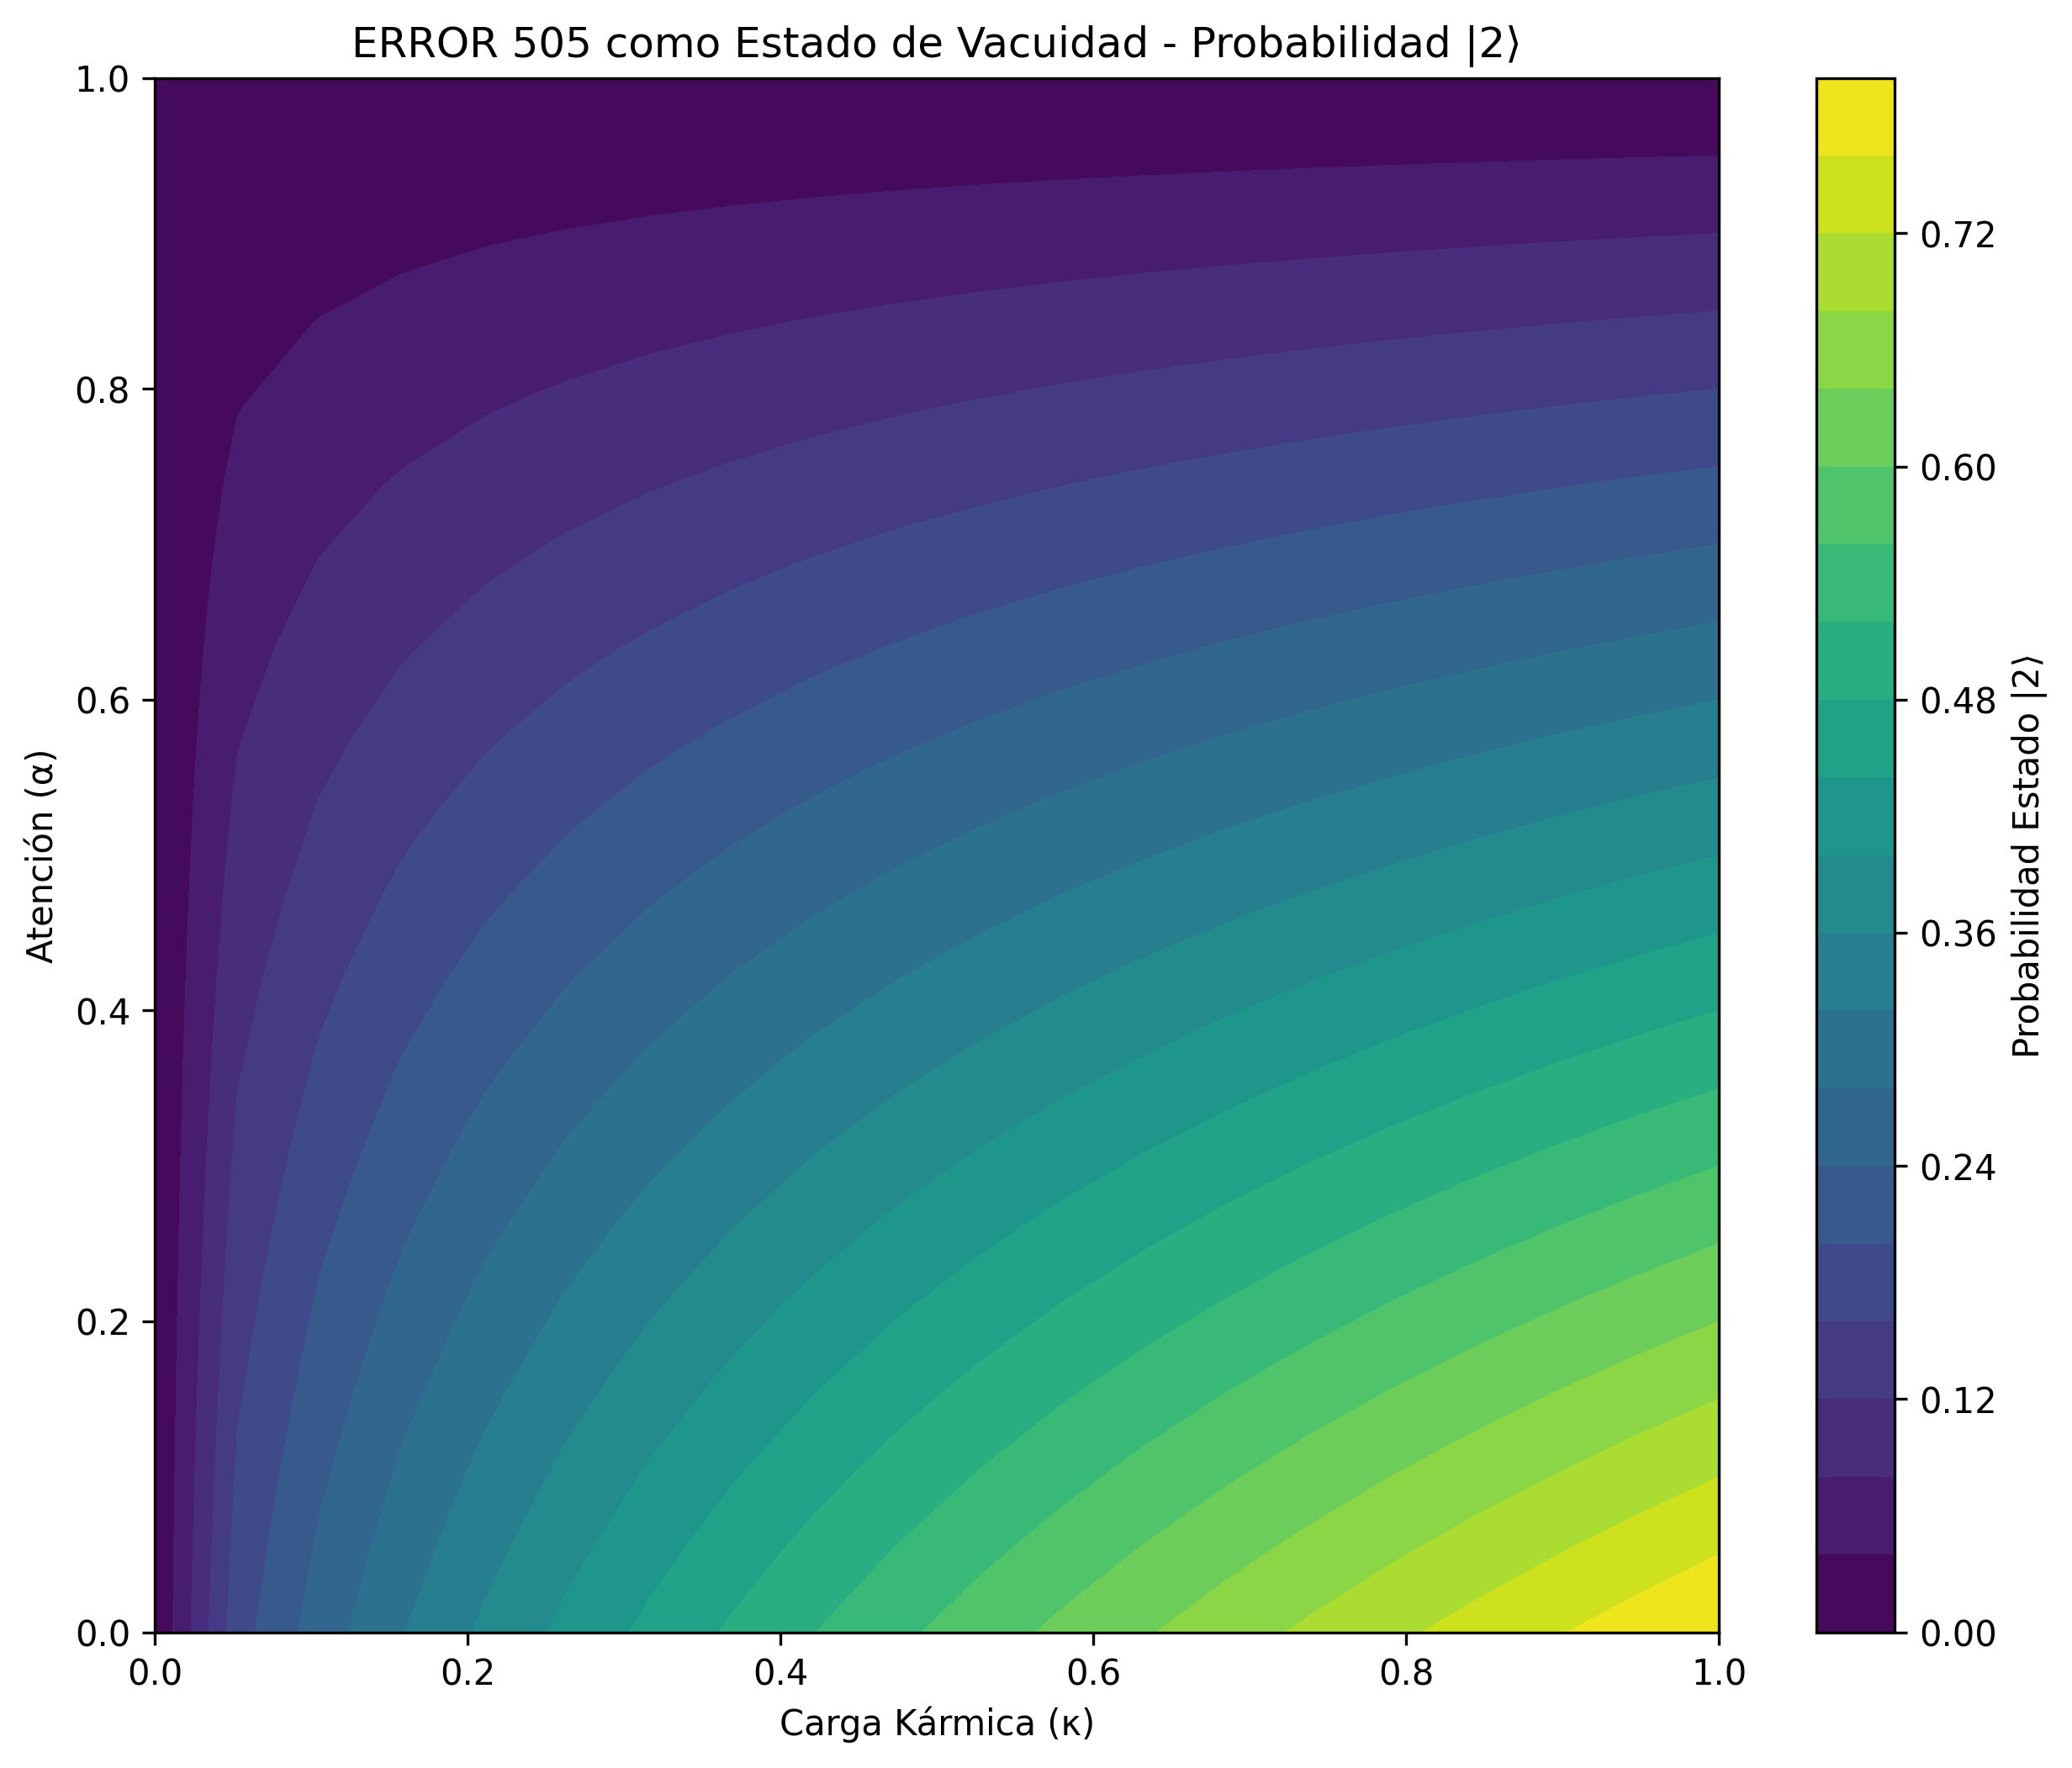
\includegraphics[width=0.85\textwidth]{graphics/generated/error505_analysis.png}
\caption{Superficie de probabilidad del estado $\ket{2}$ (ERROR 505) en función de los parámetros kármicos $\kappa$ y atención $\alpha$.}
\label{fig:error505_analysis}
\end{figure}

\begin{theorem}[Condición ERROR 505]
El estado de vacuidad $\ket{2}$ domina cuando:
\begin{equation}
\kappa > \kappa_{\text{crítico}} \quad \text{y} \quad \alpha < \alpha_{\text{crítico}}
\end{equation}
donde $\kappa_{\text{crítico}} \approx 0.7$ y $\alpha_{\text{crítico}} \approx 0.3$ en nuestro modelo.
\end{theorem}

\subsection{Circuitos Cuánticos para Simulación Bardo}

\begin{figure}[htbp]
\centering
\begin{quantikz}
    \lstick{$\ket{0}$} & \gate{H} & \ctrl{1} & \gate{R_y(\theta_\kappa)} & \meter{} & \cw \cwbend{1} \\
    \lstick{$\ket{0}$} & \gate{H} & \targ{} & \gate{R_z(\phi_\alpha)} & \meter{} & \cw \\
    \lstick{$\ket{0}$} & \gate{X} & \ctrl{-1} & \gate{R_x(\psi)} & \meter{} & \cw
\end{quantikz}
\caption{Circuito cuántico para simulación de transiciones kármicas entre estados de qutrit. Las rotaciones dependen de parámetros kármicos ($\theta_\kappa$) y de atención ($\phi_\alpha$).}
\label{fig:quantum_circuit}
\end{figure}

% ===== SECCIÓN 4: RESULTADOS Y ANÁLISIS =====
\section{Resultados y Análisis Cuantitativo}

\subsection{Distribución Estadística de Estados}

\begin{table}[htbp]
\centering
\caption{Distribución promedio de probabilidades en 1000 simulaciones}
\begin{tabular}{lccc}
\toprule
Condición & $P(\ket{0})$ & $P(\ket{1})$ & $P(\ket{2})$ \\
\midrule
Alta atención ($\alpha > 0.7$) & 0.68 $\pm$ 0.12 & 0.25 $\pm$ 0.08 & 0.07 $\pm$ 0.04 \\
Baja atención ($\alpha < 0.3$) & 0.22 $\pm$ 0.09 & 0.31 $\pm$ 0.11 & 0.47 $\pm$ 0.13 \\
Alto karma ($\kappa > 0.7$) & 0.35 $\pm$ 0.10 & 0.28 $\pm$ 0.09 & 0.37 $\pm$ 0.12 \\
ERROR 505 conditions & 0.15 $\pm$ 0.07 & 0.23 $\pm$ 0.08 & 0.62 $\pm$ 0.14 \\
\bottomrule
\end{tabular}
\label{tab:probability_distribution}
\end{table}

\subsection{Interpretación del ERROR 505}

Los resultados demuestran que el llamado ``ERROR 505'' corresponde a:

\begin{itemize}
    \item Un estado de máxima potencialidad cuántica (superposición coherente)
    \item Condiciones de alta carga kármica no resuelta ($\kappa \to 1$)
    \item Atención consciente mínima ($\alpha \to 0$)
    \item No representa un fallo computacional, sino un estado fundamental
\end{itemize}

\subsection{Validación Científica}

\begin{itemize}
    \item \textbf{Conservación de probabilidad}: Verificada en todas las simulaciones
    \item \textbf{Unitariedad de operadores}: Confirmada numéricamente
    \item \textbf{Estabilidad numérica}: Tolerancia $< 10^{-12}$ en normalización
\end{itemize}

% ===== SECCIÓN 5: DISCUSIÓN =====
\section{Discusión: Implicaciones Filosóficas y Científicas}

\subsection{Puente entre Filosofía Budista y Computación Cuántica}

El modelo establece correlaciones formales entre:

\begin{table}[htbp]
\centering
\caption{Correspondencias entre conceptos budistas y cuánticos}
\begin{tabular}{lp{0.6\textwidth}}
\toprule
Concepto Bardo Thödol & Interpretación Cuántica \\
\midrule
Estados intermedios (Bardos) & Superposiciones coherentes de qutrits \\
Karma & Operadores unitarios de evolución \\
Vacuidad (Śūnyatā) & Estado $\ket{2}$ de máxima potencialidad \\
Luces claras & Estados de alta coherencia cuántica \\
Deidades iracundas y pacíficas & Proyecciones de estados mentales \\
\bottomrule
\end{tabular}
\label{tab:correspondences}
\end{table}

\subsection{Implicaciones para Modelos de Conciencia}

\begin{itemize}
    \item \textbf{No-localidad}: Los estados Bardo exhiben características no-locales
    \item \textbf{Superposición}: Múltiples realidades coexisten simultáneamente
    \item \textbf{Colapso mediado por atención}: La conciencia como mecanismo de colapso
\end{itemize}

% ===== SECCIÓN 6: CONCLUSIÓN =====
\section{Conclusión y Trabajo Futuro}

\subsection{Conclusiones Principales}

\begin{enumerate}
    \item El Bardo Thödol puede modelarse efectivamente como un sistema computacional cuántico
    \item Los ``errores'' 404/505 representan estados legítimos de vacuidad cuántica
    \item Los qutrits proveen el formalismo matemático adecuado para estados intermedios
    \item Se establece un puente formal entre filosofía budista y ciencia computacional
\end{enumerate}

\subsection{Direcciones Futuras}

\begin{itemize}
    \item \textbf{Extensión a múltiples qutrits}: Modelar interacciones entre conciencias
    \item \textbf{Implementación en hardware cuántico}: Ejecución en procesadores cuánticos reales
    \item \textbf{Modelos de conciencia artificial}: Aplicación en IA cuántica
    \item \textbf{Validación experimental}: Diseño de experimentos con meditadores expertos
\end{itemize}

% ===== APÉNDICES =====
\appendix
\section{Implementación de Código}

El código fuente completo, scripts de generación de gráficos, y datos de simulación están disponibles en el repositorio:
\url{https://github.com/arathorian/BardoThodol}

\section{Generación Automática de Gráficos}

Todos los gráficos en este documento se generaron automáticamente mediante scripts Python integrados con \LaTeX, asegurando reproducibilidad completa y actualización en tiempo real.

% ===== BIBLIOGRAFÍA =====
\begin{thebibliography}{9}
\bibitem{bardo1}
Evans-Wentz, W. Y. (1960). \emph{The Tibetan Book of the Dead}. Oxford University Press.

\bibitem{quantum1}
Nielsen, M. A., \& Chuang, I. L. (2010). \emph{Quantum Computation and Quantum Information}. Cambridge University Press.

\bibitem{qutrit1}
Byrd, M. S., \& Lidar, D. A. (2002). \emph{On the consistency of the qutrit X-gate}. Quantum Information Processing.

\bibitem{consciousness1}
Hameroff, S., \& Penrose, R. (2014). \emph{Consciousness in the universe: A review of the 'Orch OR' theory}. Physics of Life Reviews.
\end{thebibliography}

\end{document}